\documentclass[12pt]{article}
\usepackage[margin=1in]{geometry}
\usepackage{amsmath}
\usepackage{listings}
\usepackage[utf8]{inputenc}
\usepackage{graphicx}
\usepackage{float}
\usepackage{placeins}
\usepackage{hyperref}
\usepackage{multicol}
\usepackage{caption}

\usepackage[style=alphabetic]{biblatex} 
\addbibresource{references.bib}

\author{Henry Pick \small hpick@hmc.edu \\
\large Noah Nevens \small nnevens@hmc.edu \\
\large Prakod Ngamlamai \small pngamlamai@hmc.edu}
\title{HMC Room Draw Optimization}
\DeclareMathOperator*{\maxi}{max}
\captionsetup{width=0.6\linewidth}
\begin{document}
    \maketitle
    \section*{Abstract}
    Room Draw is an annual event at Harvey Mudd College that asks returning students to select a room to live in for the following year. Students are given priority numbers and select rooms in order of their priority from the remaining available rooms. The process is often exceedingly stressful as a result of each student trying to guess what every other participant will do in order to maximize their chances of getting a room that they want. We propose an improvement on the current room draw system in the form of a multi-phase model whereby students will first be sorted into groups, then state room preferences as a group, and finally they are assigned to a room together. When we allow groups to define the amount of utility they get from certain room assignments, we found that our primary model is able to improve the assignments under every evaluation metric that we designed.
    \section*{Executive Summary}
    Under the current room draw system students feel the pressure of needing to coordinate extensively. They need to have a plan and a set of backup plans, each composed of friends to live with, a space to fit them, and some sense of security that the space won't be taken by someone else. Figuring out whom to live with, where to live, and which options are possible given what everyone else wants is a very difficult task and it makes room draw a particularly stressful time for many students. 
    
    In our case study, we present a multi-phase protocol for room assignment that aims to be nearly optimal. We assume, as a result of our experience with Harvey Mudd room draw, that students care, first and foremost, about the people they live with. As such, we choose to first formulate groups of students and have those groups act as agents throughout the remainder of the model. Those agents then state preferences for room types (e.g. single, double, triple, quad), which we collect as data. Based on these preferences, we use a linear program to assign rooms to groups of students. 

    We discuss several alternative models in the technical report, but the primary model that we want to implement is the range preference model. This model allows groups to select a range of rooms and assign them a particular utility score. Each group gets a pool of utility points that they can distribute to different room ranges (as long as they assign integer-valued utility to each range). 
    
    We simulated the current room draw system by assigning students their rooms in order of their priority numbers. Using the same generated preference data, we compared this simulation to our primary model. In what we consider a typical condition, our model improved the overall utility score by approximately $17\%$ and improved every group's chance of being assigned a room in one of their higher preferences. This is an improvement that we consider worthy of implementation. Ideally, the model and the interfaces together can be implemented in the near future. 
    
    \section*{Technical Report}
    \subsection*{Introduction}
    For many students at Harvey Mudd, room draw is the most stressful time of the year. It's very difficult to coordinate your choice with that of all the other students vying for the same spot. Participants typically have a list of preferences prior to the draw, but many times they end up with none of their top choices because of how chaotically the event pans out. 
    
    We can gather information about students' preferences, including preferred dorm, room type, group they'd live with, etc. This motivates the creation of a model that uses this data to optimize the room draw problem that plagues so many students year to year. For the purposes of our project we created a multi-phase model to collect data, match roommates and assign rooms. We break down each of these phases below: 

        \subsubsection*{Phase 1: Roommate Matching}
    The first stage of the protocol asks students to state preferences for whom to live with and what room type they'd prefer to live in. Under the current room draw system, students are assigned priority numbers. Students with higher priority numbers can secure an available room before students with lower priority numbers. Under our system, students with higher priority numbers will be able to unilaterally decide whom they will live with according to their preferred room type, \textit{but} their priority number will not grant them earlier access to preferred rooms. Therefore, there is really no incentive to simply group with high priority friends because priority numbers don't influence room assignment in our model.
    
    We are currently developing a user interface that students can use as a form to select a desired room type and then write in names of desired roommates. We plan to allow students to state three distinct preferences on the form. For each preference, the student names their desired room type (which include rooms within a suite) and then lists a number of desired roommates according to their rooming plans.
    
    This model assumes that students care more about whom they live with than which specific room they live in. In the event that a student cares more about their specific room assignment than the people they live with (an exceedingly rare case), they will be in a group by themself. That way, if a student's first preference is a triple with students A and B but their second preference is a different room type with different students, then they can state their desires at that level of complexity. 
    
    Finally, we assign high priority students to their highest available room type and roommate preference, where available means that their desired roommates are not already taken and there are enough rooms of their desired room type to house them and all of the higher priority students who have already been assigned that room type.
    
    \subsubsection*{Phase 2: Stating Preferences as a Group} 
    The next stage of the procedure does not involve an algorithm. Rather, we ask students to fill out another form, but this time they will do so as a group (specifically, the group they were assigned as per the previous phase). Each group must live in the room type that they were assigned as a result of the first phase.
    
    This new form, which is currently under development, will ask each group of students to state their room preferences. It will first ask them to state a desired dorm, and then generate a list of floors according to the number of floors in that dorm. Each group is given a quota of $100$ utility points which they can now assign to rooms using this form.

    In the case of our primary model, the range preference model, students will assign utility scores to a range of rooms. The students choose the range and an integer-valued utility to assign. Any room that is not included in any of the preferred room ranges represents $0$ utility for that group.
    
    \subsubsection*{Phase 3: The Linear Program} 
    The linear program assigns groups to rooms in a way that maximizes utility for all participants. Each room has a specified capacity and the group size assigned to the room cannot exceed that capacity.  When a group is matched to a room range, every room in that range must have a capacity large enough for the group. Note that suites (in the case of Atwood, Linde and Drinkward) are not considered different from consecutive individual rooms in our model. 
    
    We introduce multiple slightly different linear programs and test to determine the best way to perform our room assignment. They primarily differ in the number and type of preferences they allow students to make. Each model will be discussed in full in the following section, but the model we ultimately choose is the one that coincides exactly with the three stages as they have been outlined in this summary. 
    
    In the next section we will give the formulations for several model candidates and variations of our final model. Before doing so, we will briefly overview each model and mention what distinguishes it from the others:

    \begin{enumerate}
        \item The \textbf{single preference} model allows each group of students to state only one room preference. This model is not final since it does not take full advantage of our second phase, which allows students to make multiple preferences. 
        \item The \textbf{multi preference} model allows groups to state multiple preferences. 
        \item The \textbf{range preference} model is our primary model. Groups can select a range of rooms (e.g. rooms 15-21) and list them as a particular preference. Since all the rooms in a particular area have similar numbers, this allows groups to select an entire suite as part of their range. In fact, it allows multiple groups to be placed in a suite and, further, for them to be correctly sorted in the rooms of that suite. However each room within that suite can only receive one group of students. So a group of one and a group of two cannot make up a triple. But unlike the previous two models, a group of three and a group of two can both be in a suite provided there is a triple and a double in those groups' respective ranges.
        \item The \textbf{min cost flow} model transforms the final phase of the model into a variant of the minimum cost flow problem. All the groups are fixed and can flow into rooms. Each room has a capacity and the cumulative sizes of the groups that flow into a room cannot exceed the capacity. 
        \item The \textbf{maximin} model maximizes the utility of the student group that is worse off. One of the drawbacks of utility-maximizing models is that they can cause one agent to receive a tragically low utility. In an effort to humanize our results, we will also discuss the utility earned by the worst-off student for our primary model as part of our post-optimality analysis. 
    \end{enumerate}
    
   We find that the range preference model gives us the most flexibility because it allows groups to assign utility scores to ranges of rooms. This makes it so that if a group fails to, for instance, obtain a double on a certain floor, they can obtain the vacant double right next to it without having to explicitly state a separate preference for that alternate double. 
   
   All of the models make improvements on the current room draw system, but the range preference model allows the most flexibility and the ranges are more accurate to what we think students will prefer. 
   
   The next subsection will show the formulation for each of the four models we just outlined. We will then describe the results of running each model and how they compare to a simulation of the current room draw system using the same data. These results will help us argue in favor of replacing the current room draw system with ours. We will explain why we believe we can actually implement our model and then describe the next steps we need to take before doing so. 
    
    \subsection*{Model Formulation}
    We implement the third phase of the process with the following models, which all maximize the total sum of utility.
    \subsubsection*{Single Preference Model}
    Let $G$ be the set of participant groups in Room Draw. \\
    Let $R$ be the set of rooms, where $|R| = |G|$ \\
    Let $P_r$ be the preference rank, which in the single preference model has only one element $P_r =\{1\}$. \\
We have the following parameters: $w_{pr}$ the weight of preference rank $pr$ and $p_{g,pr}$ the preference with rank $pr$ of a particular group $g$. \\
    We define the following decision variables: $s_{g,pr}$ a binary variable indicating whether preference $pr$ of group $g$ is met, and $a_{g,r}$ the binary variable indicating assignment of group $g$ to room $r$. 
    \begin{align*}
    \text{Max} &\sum_{g \in G, pr \in P_r} s_{g,pr}w_{pr}  & \\
    \text{Subject to } &s_{g,pr} = a_{g,p_{g,pr}} &\forall g \in G, pr \in P_r\\ 
    &\sum_{g \in G} a_{g,r} = 1 &\forall r \in R
    \end{align*}
    where the first constraint checks whether, for a group $g$, their $pr^{\text{th}}$ preference, which in this case is their only preference, is satisfied through assignment. \\
    The second constraint forces each room to accept only one group, which in turn implies that each person can only get into one room.
    
    \subsubsection*{Multi Preference Model}
    This model is applicable when there is more than one preference in the set $P_r$. It uses the same sets and parameters as the previous model.\\
%    Let $G$ be the set of participant groups in Room Draw. \\
%    Let $R$ be the set of rooms, where $|R| = |G|$ \\
%    Let $P_r$ be the set of preference ranks. \\
%We have the following parameters: $w_{pr}$ the weight of preference rank $pr$ and $p_{g,pr}$ the preference with rank $pr$ of a particular group $g$. \\
%    We define the following decision variables: $s_{g,pr}$ a binary variable indicating whether preference $pr$ of group $g$ is met, and $a_{g,r}$ the binary variable indicating assignment of group $g$ to room $r$. 
    
    \begin{align*}
    \text{Max} &\sum_{g \in G, pr \in P_r} s_{g,pr}w_{pr}    \\
    \text{Subject to } &s_{g,pr} = a_{g,p_{g,pr}} &\forall g \in G, pr \in P_r\\ 
    &\sum_{g \in G} a_{g,r} = 1 &\forall r \in R
    \end{align*}
    where again the first constraint checks whether, for a group $g$, their $pr^{\text{th}}$ preference (represented by $p_{g,pr}$) is satisfied through assignment. In which case $s_{g,pr} = 1$. \\
    The second constraint forces each room to accept only one group, which implies that each person can only get into one room.


    \subsubsection*{Range Preference Model}
    This model allows groups to select a range of rooms and assign it a utility weight. We can slightly modify the previous models by adding a few parameters. \\
%     Let $G$ be the set of participant groups in Room Draw. \\
%    Let $R$ be the set of rooms, where $|R| = |G|$ \\
%    Let $P_r$ be the set of preference ranks. \\
We add the following parameters: $pl_{g,pr}$ the lower bound of the preference range with rank $pr$ of a particular group $g$, and $pu_{g,pr}$ the upper bound of the preference range with rank $pr$ of a particular group $g$\\
%$w_{pr}$ the weight of preference rank $pr$, $pl_{g,pr}$ the lower bound of the preference range with rank $pr$ of a particular group $g$, and $pu_{g,pr}$ the upper bound of the preference range with rank $pr$ of a particular group $g$\\
%    We define the following decision variables: $s_{g,pr}$ a binary variable indicating whether preference $pr$ of group $g$ is met, and $a_{g,r}$ the binary variable indicating assignment of group $g$ to room $r$. 
    
    \begin{align*}
    \text{Max} &\sum_{g \in G, pr \in P_r} s_{g,pr}w_{pr}  & \\
    \text{Subject to } &s_{g,pr} = \sum_{r = pl_{g,pr}}^{pu_{g,pr}} a_{g,r} &\forall g \in G, pr \in P_r\\ 
    &\sum_{g \in G} a_{g,r} = 1 &\forall r \in R
    \end{align*}
    where again the first constraint checks whether, for a group $g$, their $pr^{\text{th}}$ preference range (represented by the range of the sum $\sum_{r = pl_{g,pr}}^{pu_{g,pr}}$) is satisfied through assignment $a_{g,r}$. In which case $s_{g,pr} = 1$. \\

    

    
    \subsubsection*{Minimum Cost Flow Model}
    This model treats the process as a minimum cost flow problem, where cost refers to the negative of utility.
%    Let $G$ be the set of participant group
%    Let $R$ be the set of room sets, which is a collection of rooms of particular characteristic.
    Let $L$ be the set of edges or links between $G$ and $R$.
    We have the following parameters: $u_{g,r}$ the utility of the link between $g \in G$ and $r \in R$, $c_r$ the capacity of room set $r$, and $s_g$ the size of group $g$. 
%    We define the following binary decision variable $a_{g,r}$ indicating whether the group $g$ is assigned to room set $r$.
    
    \begin{align*}
        \text{Max} &\sum_{(g,r) \in L} u_{g,r}a_{g,r} &\\
        \text{Subject to } &\sum_{g \in G} a_{g,r}s_g \leq c_r 
        & \forall r \in R \\
        &\sum_{r \in R} a_{g,r} = 1 & \forall g \in G
    \end{align*}

    where the first constraint represents the room capacity requirement and the second constraint forces the group to be assigned to only a single room.

    \subsubsection*{Maximin Model}
    This model maximizes the utility earned by the student group that is worst off. The sets and parameters are the same as the range preference model, except that we have a decision variable $v$ that represents the utility of the worst-off student.

    \begin{align*}
    \text{Max } &v \\
    \text{Subject to } &s_{g,pr} = \sum_{r = pl_{g,pr}}^{pu_{g,pr}} a_{g,r} &\forall g \in G, pr \in P_r\\ 
    v &\leq \sum_{pr \in P_r} s_{g,pr}w_{pr} &\forall g \in G\\
    &\sum_{g \in G} a_{g,r} = 1 &\forall r \in R
    \end{align*}

    Note that we have the same constraints as the range preference model, but we have added one to ensure $v$ is always less than the total utility earned by any one student. That way, we are truly maximizing the minimum utility. 

    \subsection*{Results}
    \FloatBarrier
    We compare the results from the range preference model against a priority number model using shared randomly generated data sets and utility calculations. The priority number model represents a simplified version of the current room draw process, where every participant is assigned a priority number and each chooses in a way to maximize their own utility when it is their turn. The details of this model can be found in Appendix B. A typical performance comparison between the optimized and greedy module is shown in Figure \ref{fig:preference_satisfaction}. Across multiple simulations of randomly generated data, we also compiled summary statistics that give a better sense of the model's expected performance in Figure \ref{fig:summary_stats}.
    \begin{figure}[h]
        \centering
        \begin{multicols}{2}
            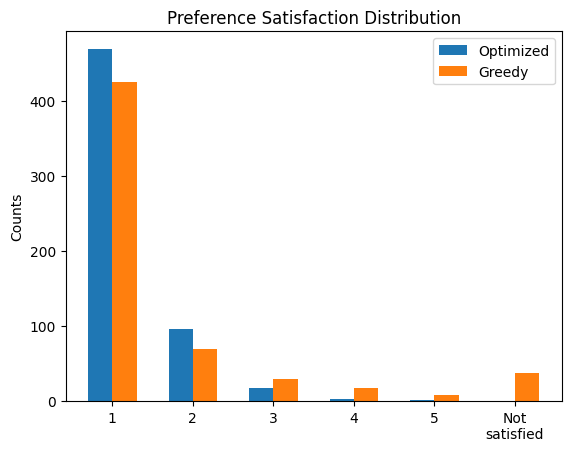
\includegraphics[width=\linewidth]{res/preference_satisfaction_comparison.png}

\caption{Comparison of the assignment performances of the optimized and priority (greedy) models. Number of groups receiving each preference rank are shown where each group has 5 preferences of maximum range 20.}
        \label{fig:preference_satisfaction}
             
      \columnbreak      

      Preference Satisfaction Counts
            \begin{tabular}{c|cc}
                Preference & Un-optimized & Optimized \\
                \hline
                1 & 425 & 469\\
                2 & 69 & 96\\
                3 & 30 & 17\\
                4 & 17 & 3\\
                5 & 8 & 2\\
                \hline
                Unsatisfied & 38 & 0
            \end{tabular}
        \caption{Tabular data for the comparison. Un-optimized column refers to the priority (greedy) model while the Optimized column refers to the range preference model.}
        \label{fig:tabulardata}
        \end{multicols}
    \end{figure}

    \begin{figure}[h]
        \centering
        \captionsetup{width=.7\linewidth}
        Improvement Summary Statistics
        
        \begin{tabular}{cccc}
            Tot. Util. Improvement \% & Pref 1 & Pref 2 & Not satisfied\\
            \hline
            $17\pm1.3\%$ & $40\pm 2.8$ & $29\pm 9.6$ & $-39\pm5.2$
        \end{tabular}
        
        \caption{Summary statistics for model performance when and \texttt{n\_preferences = 5} and \texttt{max\_range = 20}, which are the established ``typical'' preference conditions. Total utility improvement indicates the overall utility improvement percentage between priority and optimized models. Pref 1, Pref 2 and Not satisfied are the expected changes for preference satisfaction counts.}
        \label{fig:summary_stats}
    \end{figure}

    \subsubsection*{Sensitivity Analysis}
    Because our program is an integer program, performing sensitivity analysis will take a different form than the traditional assessment of constraint sensitivity. We instead focus on the parameters used in the data generation to see how the optimization model performs. The two parameters of concern are the number of preferences of each group and the width of each preference range (i.e. the maximum number of rooms that a group can assign to each preference range). These parameters correspond to varying degrees of how particular groups are about their room assignments. Fewer preferences and smaller preference width mean that the preferences of each group will be more difficult to satisfy individually.

    Each data point in these tests was collected by sampling four simulation runs to estimate the mean and variance of the improvement. Rather than plotting the absolute utility sum of the models, we computed the performance improvement over the priority draw---a better indicator of the model's qualitative performance. Figure \ref{fig:maxrange} shows the sensitivity of the model with respect to the maximum width of each preference range. A general trend in sensitivity here is inconclusive, however it does appear that for a max preference range of greater than 5, the performance improvement relative to the priority model remains constant.
    \begin{figure}[h]
        \centering
        \captionsetup{width=.7\linewidth}
        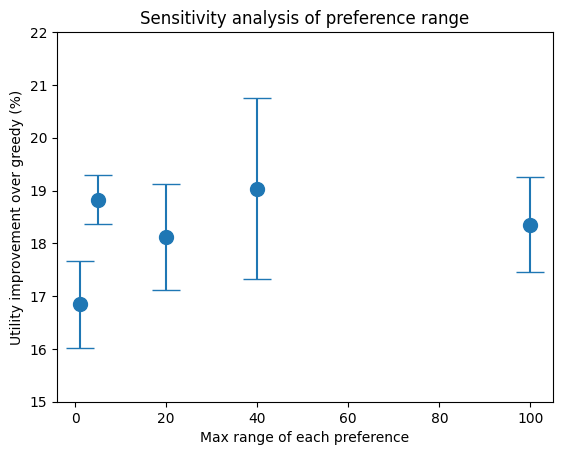
\includegraphics[width=0.55\linewidth]{res/range_sensitivity_analysis.png}
        \caption{Improvement of utility value in percentage over varying maximum range parameter (1, 5, 20, 40, 100). The error bars denote the standard deviations of the four data points.}
        \label{fig:maxrange}
    \end{figure}

    Figure \ref{fig:numpref} summarizes the sensitivity analysis with respect to the number of preferences that each group is allowed to specify. We chose values ranging in between 1 and 5, which we assume reasonably encapsulates the number of preferences that a typical student would have during the draw. A more identifiable trend is evident here in the downward correlation between the number of preferences and relative performance with the priority model.
    \begin{figure}[h]
        \centering
        \captionsetup{width=.7\linewidth}
        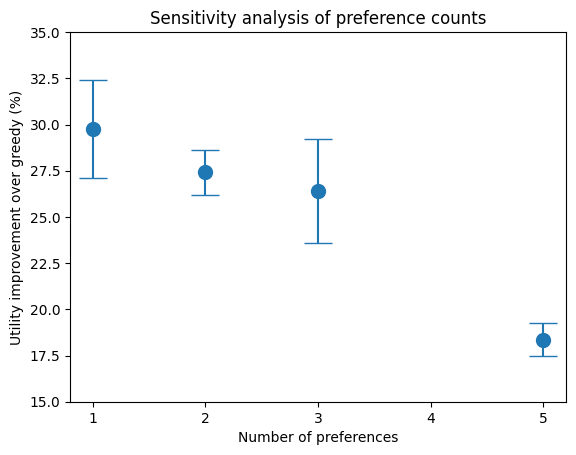
\includegraphics[scale = 0.65]{res/num_prefs_sensitivity_analysis.png}
        \caption{Improvement of utility value in percentage over varying number of preferences. The error bars denote the standard deviations of the four data points.}
        \label{fig:numpref}
    \end{figure}


    
    \FloatBarrier
    \subsection*{Conclusion}
    As can be seen from Figures \ref{fig:preference_satisfaction} and \ref{fig:tabulardata}, when every agent states five preferences, our model grants one of those five preferences to every group. This is much better than the priority number model, which leaves $38$ (or $6.5\%$) of students with a room that they gave no utility to. Additionally, under our model students were granted their first and second choice rooms far more frequently than in the priority number model. 

    As can be seen from Figure \ref{fig:maxrange}, the ability to select a range of rooms clearly offers increased utility when the maximum allowable size of the range is greater than $1$. But it seems that utility improvement tapers off after a maximum allowable range size of $5$ or so. In general, the average improvements is noticeable over all maximum range value.

    With Figure \ref{fig:numpref}, the improvement of the range preference model over the priority number model is most noticeable at extremely low number of preferences. However, we see that all the values of the number of preferences still offer significant improvements. 
    
    We conclude that the range preference model is fairly accurate with respect to the complexities of room draw and only makes simplifying assumptions in cases where it is justified in doing so. We also observe that the range preference model has stable solution values across different preference data and is a consistent improvement on the priority number model in both total utility and the number of students having their higher preferences met.
    Since we see such a significant improvement across multiple data sets, we believe that our model is suitable for implementation in real life. In order to make this happen, we plan to finish developing the user interfaces that will allow us to collect preference data from students. We believe that the flexibility of choices available by forms, the multiple phases in our algorithm, and the relational database we're developing will be worthy of implementation.
    \FloatBarrier
    
    \section*{Appendix}
    \subsection*{A: Data Sets}
        Our data file is far too large for LaTex, but we have it stored in preferences.md on the model-tests branch of our GitHub repository:
        https://github.com/henry-2025/room-draw-optim/tree/model-tests

        In order to do probabilistic sensitivity analysis, we created a random preference generator that creates tables like the one in the data file and feeds them into the model via AMPL's python API. The following pseudocode describes this generation
\begin{lstlisting}[language=python]
#### PARAMETERS, adjusted in sensitivity analysis ###

#number of rooms
n_rooms = 587
n_groups = n_rooms
# number of preference points assigned to each person
pref_tot = 100
# number of preferences
n_pref = 5
# max preference range that each preference has
max_range = 20

# preference and weight parameters
# a matrix of rows sorted in descending order whose sums
# are all equal to pref_tot
weights = norm_rows(sort_rows(random((n_groups,n_pref))), pref_tot) 

# important: we cannot have overlapping preferences,
# which makes preference generation sort of tedious
pref_lower = zeros((n_groups, n_pref))
pref_upper = zeros((n_groups, n_pref))
for i in range(n_groups):
    # get three distinct, but otherwise random rooms
    # and assign those as the lower range bounds
    pref_queue = range(1, n_rooms + 1, 1)
    shuffle(preference_queue)
    pref_lower[i,:] = sort(pref_queue[:n_preferences])

    # assign the upper range bounds, ensuring that they
    # don't overlap with other preferences for that person
    for j in range(n_pref-1):
        pref_upper[i,j] = min(pref_lower[i,j] + 
            randint(0, n_preferences), pref_lower[i,j+1])
    pref_upper[i,n_pref-1] = min(pref_lower[i,n_pref-1] + 
        randint(0, n_pref), n_rooms)

    # permute the preferences so they are no longer
    # strictly ordered
    permute = permutation(n_preferences)
    preferences_lower[i,:] = preferences_lower[i,permute]
    preferences_upper[i,:] = preferences_upper[i,permute]
\end{lstlisting}


    
    \subsection*{B: Priority Number Model Code}
    \begin{lstlisting}[language=python]
assignment = np.zeros(n_people, dtype=np.int32)
weight = np.zeros(n_people, dtype=np.int32)
for person in range(n_people):
    assigned = False
    for pref in range(n_preferences):
        for i in range(preferences_lower[person, pref]-1, \
        preferences_upper[person, pref]):
            if not assignment[i]:
                assigned = True
                assignment[i] = person
                weight[i] = n_preferences - pref
                break
        if assigned:
            break
    if not assigned:
        for i in range(n_rooms):
            if not assignment[i]:
                assignment[i] = person
                break
    \end{lstlisting}





    \nocite{*}
    \printbibliography[title = Bibliography]
    
%    \section{TODO}
%    \begin{enumerate}
%        \item Delete TODO section
%        \item do more proofreading
%        \item executive summary is too long, shorten and put more technical information into model description
%        \item Postoptimality analysis:
%        \begin{enumerate}
%            \item Figure out how we are expected to do this with an assignment model
%            \item Possibly by increasing the number of preference ranks (the size of $P_r$), or 
%            \item Change the number of utility points quota that each student can allocate. (Would result in no change for single preference, but can potentially result in change for multi preference etc.)
%            \item do statistics (ANOVA) for each size of $P_r$.
%        \end{enumerate}
%        \item Maximin as objective function
%    \end{enumerate}
    
\end{document}